\section{Introduction}

\mbox{}\\

Leap Motion is the device that allows user to communicate with the master device using set of gestures. The controller is based on two monochromatic IR cameras and infra red LEDs which allows it to detect movement on distance around 1 meter. Hands and gestures detected by sensor are send as frames in number around 200 per second, which are used later by the device program localised on the master device. Although the technology is being sold from 2012, the device is not working sufficiently satisfactory.Numerous problems may be found during usage, as problems with detecting smaller hands, confusing left and right hand or misidentifying the extended fingers. \\

Considering above informations, the main aim of the project was to create application, which using newly designed gestures would allow user to communicate and control robot arm. According to that, the main idea of presented application is the idea of writing robot, which could be used to write, draw or follow user hands on any surface, and in any size, especially in hazardous and contaminated environment, which would not be safe or available for operator access. In order to correct the accuracy and quality of gesture recognition, additional mean filter has been applied.\\

To achieve the objectives, two individual modes were created. The first, static mode, for detecting gestures which would correspond 
to a certain letter from letters library. The second mode, based on dynamic detection of users' hand movement, which is followed by robot's arm. \\

Application starts with mode selection, using set of gestures presented in Figure \ref{fig:mode}, after which certain mode is activated, but can be switched at any time of operating. 


\begin{figure}[H]
	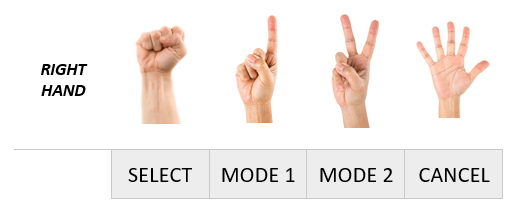
\includegraphics{mode_selection}
	\centering
	\caption{Mode selection - set of gestures}
	\label{fig:mode}
\end{figure}


The application is dedicated to used Universal Robot arm, which is easy to cooperate with and offers fast configuration, but could be applied to any similar working robot. Communication is realised by certain part of program, which will be described thoroughly in following report. To allow most optimal and full application usage, robot operation is realised by set of function written in C++, instead of program dedicated to the robot by producer. 
